\documentclass[]{subfiles}

\begin{document}
\section{Be(nuts)eranleitung}
\subsection{Installation}
	\subsubsection{Installationsvoraussetzungen}
	NUTS2.0 sollte sich auf jedem Betriebssystem ausführen lassen.
	Für die Ausführung wird eine Python 3.7 installation (oder aktueller) benötigt.
	Diese kann unter https://www.python.org/downloads/ heruntergeladen werden.

	Um NUTS2.0 ausführen zu können, muss zuerst das Github-Repository geklont werden:\\
	https://github.com/EkoGuandor229/Network-Unit-Testing. 
	Danach können die verwendeten Module über das Requirements-File mit dem Befehl
	'pip install -r requirements.txt' installiert werden.

	\subsubsection{Ausführen}
	Das Programm kann zu Testzwecken regulär in einer Programmierumgebung 
	wie zum Beispiel PyCharm ausgeführt werden.

	Um NUTS2.0 aus einer Konsole zu starten muss zum Root-Ordner NUTS2.0 navigiert werden. 
	Z.B. C:/Programs/Python/NUTS2.0.

	Man kann das Programm mit dem Befehl: 'python -m nuts' starten. 
	Wenn man das GUI auslassen und direkt alle Tests ausführen möchte kann
	man mit dem Befehl: 'python -m nuts -r' starten.

	\subsubsection{Konfiguration}
	Im File 'config.yaml' können die Pfäde aller Ordner geändert werden, um beispielsweise
	das Inventory oder die Resultate zentral in einem Repository zu verwalten. 
	Zusätzlich kann noch bestimmt werden, ob das GUI Per default übersprungen werden soll.

	\newpage

\subsection{Inventar}
	Um Netzwerktests auszuführen benötigt man zuerst ein Inventar mit Devices und 
	Device Connections.
	Die Devices sind die Netzwerkgeräte wie zum Beispiel Router oder Switches.
	Die Device Connections sind die Verbindungen zwischen den Devices.

	\subsubsection{Devices}
		Die Definitionen der Devices sind unter Resources/Inventory/Devices/devices.yaml abgelegt:

		\begin{figure}[h!]
			\begin{center}
				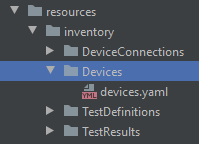
\includegraphics[scale=0.8]{\vorlagenOrdner/Bilder/Manual/Devices_yaml.png}
				\caption{Position devices.yaml}
			\end{center}
		\end{figure}

		Um neue Devices zu erfassen müssen Informationen gemäss der Tabelle~\ref{table:Deviceparameter} im yaml eingegeben werden:\\
		\begin{table}[h!]
			\begin{tabularx}{\textwidth}{lX}
			\toprule
			Attribut & Beschreibung \\
			\midrule
			device\_id & Eine eindeutige ID für das Device \\
			platform & Das OS welches das Device benutzt \\
			username & Der username welches das Device für das Login benutzt\\
			password & Das Passwort welches das Device für das Login benutzt\\
			hostname & Die Ip Adresse über welche das Device angesprochen werden kann\\
			loopback-addresse & IP-Addresse des Loopback-Interface. Für einige Tests benötigt.\\
			\midrule
			\end{tabularx}
			\caption{Deviceparameter}
			\label{table:Deviceparameter}
		\end{table}
		
		Diese Informationen sollten wie in der Abbildung~\ref{fig:DeviceErfassung} dargestellt werden: 

		\begin{figure}[h!]
			\begin{center}
				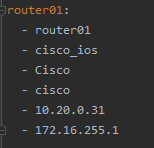
\includegraphics[scale=0.8]{\vorlagenOrdner/Bilder/Manual/Devices.png}
				\caption{Beispiel-Erfassung Device}
				\label{fig:DeviceErfassung}
			\end{center}
		\end{figure}

	\newpage

	\subsubsection{Device Connections}
		Die Definitionen der Device Connections sind unter 
		Resources/Inventory/DeviceConnections/deviceConnections.yaml abgelegt

		\begin{figure}[h!]
			\begin{center}
				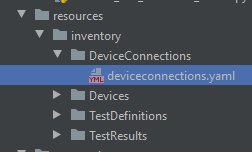
\includegraphics[scale=0.8]{\vorlagenOrdner/Bilder/Manual/DeviceConnections_yaml.png}
				\caption{Position deviceconnections.yaml}
			\end{center}
		\end{figure}

		Um Device Connections zu erfassen müssen Informationen gemäss der Tabelle~\ref{table:DeviceConnectionParameter} im yaml eingegeben werden:

		\begin{table}[h!]
			\begin{tabularx}{\textwidth}{ll}
			\toprule
			Attribut & Beschreibung \\
			\midrule
			device a & Die ID des ersten Devices \\
			device b & Die ID des zweiten Devices \\
			connection speed & Die Übertragungsrate der Verbindung\\
			\midrule
			\end{tabularx}
			\caption{DeviceConnection Parameter}
			\label{table:DeviceConnectionParameter}
		\end{table}
		

		Diese Informationen sollten wie in der Abbildung~\ref{fig:ErfassungConnection} dargestellt werden: 

		\begin{figure}[h!]
			\begin{center}
				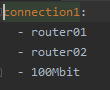
\includegraphics[scale=1.0]{\vorlagenOrdner/Bilder/Manual/DeviceConnections.png}
				\caption{Beispiel-Erfassung Connection}
				\label{fig:ErfassungConnection}
			\end{center}
		\end{figure}

		\newpage

\subsection{Netzwerktests}
	Die Netzwerktests sind die Tests, welche effektiv auf dem zu testenden Netzwerk 
	ausgeführt werden sollen.
	Die Testdefinitionen befinden sich unter Resources/Inventory/TestDefinitions:

	\begin{figure}[h!]
		\begin{center}
			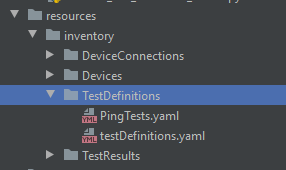
\includegraphics[scale=1.0]{\vorlagenOrdner/Bilder/Manual/TestDefinitions_yaml.png}
			\caption{Position Testdefinitionen}
		\end{center}
	\end{figure}


	Es können in diesem Ordner beliebig viele YAML Files abgelegt werden und es werden vonn allen Files die Tests erfasst.

	Um die Tests zu erfassen müssen Informationen gemäss der Tabelle~\ref{table:TestDefinitionParameter} im yaml eingegeben werden:

	\begin{table}[h!]
		\begin{tabularx}{\textwidth}{ll}
		\toprule
		Attribut & Beschreibung \\
		\midrule
		test\_id & Eine eindeutige ID für den Test \\
		command & Ein Command um den Test zu bestimmen \\
		test\_device & Die ID des Devices auf welchem der Test ausgeführt werden soll\\
		target & Das Ziel (Zum Beispiel eine IP im Falle eines Pings)\\
		expected\_result & Das erwartete Resultat (Zum Beispiel Success im Falle eines Pings)\\
		test\_group & Ein Gruppenname um später die Tests zu Kategorisieren\\
		\midrule
		\end{tabularx}
		\caption{Testdefinition Parameter}
		\label{table:TestDefinitionParameter}
	\end{table}
	

	Diese Informationen sollten wie in der Abbildung~\ref{fig:TestDefinitionErfassung} dargestellt werden: 

	\begin{figure}[h!]
		\begin{center}
			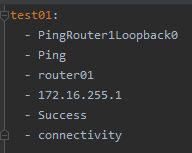
\includegraphics[scale=1.0]{\vorlagenOrdner/Bilder/Manual/TestDefinitions.png}
			\caption{Beispiel-Erfassung Testdefinition}
			\label{fig:TestDefinitionErfassung}
		\end{center}
	\end{figure}
	\newpage

	\subsubsection{Commands}
		Folgende Commands sind bereits implementiert und können mit den jeweiligen expected\_results verwendet werden:
		\paragraph*{Ping}
			Führt einen Ping-Test auf das spezifizierte Target mit 4 ICMP Packeten aus.
			In der jetzigen Konfiguration wird eine 100\% Erfolgsquote erwartet, 
			damit der Ping-Test als erfolgreich gilt.
			Wenn andere Werte erwartet werden, muss dafür ein neuer Ping-Test implementiert
			werden, welche unterschiedliche Erwartungswerte implementiert hat.

			Als erwartetes Resultat kann 'Success' oder 'Failure' verwendet werden.

		\paragraph*{Show Interfaces}
			Der 'Show Interfaces'-Befehl benötigt kein Target, da die Interfaces des test\_device
			abgefragt werden. 
			Bei der Definition kann somit einfach 'No Target' eingegeben werden.
			Als erwartetes Resultat wird ein Dictionary mit key:'Interfacename' und 
			value:'True' oder 'False' verwendet werden.
			Dies sollte gemäss der Abbildung~\ref{fig:ShowInterfacesErwarungswert}:

			\begin{figure}[h!]
				\begin{center}
					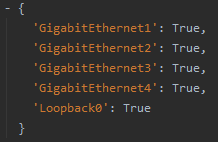
\includegraphics[scale=1.0]{\vorlagenOrdner/Bilder/Manual/ShowInterfaces.png}
					\caption{Show Interfaces Erwartungswert}
					\label{fig:ShowInterfacesErwarungswert}
				\end{center}
			\end{figure}

		\paragraph*{Traceroute}
			Führt einen Traceroute vom test\_device auf das in target angegebene Ziel aus.
			Als erwartetes Resultat wird ein Array von IP Adressen angegeben.
			Diese müssen in der Reihenfolge, in denen die Hops im Traceroute besucht werden,
			angegeben werden. Für Hops, die keine IP-Addresse anzeigen, kann ein '*' in das
			Array eingetragen werden.

			Das Array bei expected\_result kann beispielsweise so aussehen:

			\begin{figure}[h!]
				\begin{center}
					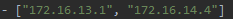
\includegraphics[scale=1.0]{\vorlagenOrdner/Bilder/Manual/Traceroute.png}
					\caption{Traceroute Erwartungswert}
				\end{center}
			\end{figure}

		\paragraph*{Arp Table}
			Für den Befehl 'Arp Table' wird kein Target benötigt, 
			da der Arp Table des im test\_device angegebenen Netzwerkgeräts abgefragt wird. 
			Es kann 'No Target' im 'target'-Feld eingegeben werden.
			Als erwartetes Resultat wird ein Array von Dictionaries erwartet. 
			In den Dictionaries werden folgende Informationen erwartet:

			\begin{table}[h!]
				\begin{tabularx}{\textwidth}{lX}
				\toprule
				Parametername & Parameterwert \\
				\midrule
				'interface': &  Name des Interface. \\
				'mac': &  MAC-Addresse des Nachbargeräts \\
				'ip': & IP-Addresse des Nachbargeräts \\
				\bottomrule
				\end{tabularx}
				\caption{ARP Table Erwartungswert Parameter}
			\end{table}
			

			In Abbildung~\ref{fig:ARPTableErwartungswert} ist ein Beispiel des Arrays mit den Dictionaries in jeder Zeile angegeben:

			\begin{figure}[h!]
				\begin{center}
					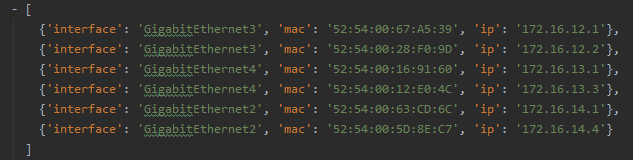
\includegraphics[scale=0.8]{\vorlagenOrdner/Bilder/Manual/ArpTable.png}
					\caption{ARP Table Erwartungswert}
					\label{ARPTableErwartungswert}
				\end{center}
			\end{figure}

		\paragraph*{Ospf Neighbor}
			Für den Befehl 'Ospf Neighbor' wird kein Target benötigt, 
			da OSPF Nachbarn des im test\_device angegebenen Netzwerkgeräts abgefragt wird. 
			Es kann 'No Target' im 'target'-Feld eingegeben werden.	
			Als erwartetes Resultat wird ein Array mit Dictionaries erwartet. 
			In den Dictionaries werden Informationen gemäss der Tabelle~\ref{table:OSPFErwartungswert}benötigt:

			\begin{table}[h!]
				\begin{tabularx}{\textwidth}{lX}
				\toprule
				Parametername & Parameterwert\\
				\midrule 
				'Neighbor-ID': & IP-Addresse des Nachbargeräts \\
				'Priority': & OSPF-Priorität als Ganzzahl\\
				'State': & Status des Nachbargeräts \\
				'Address': & IP-Addresse des Interface, über welches der Nachbar erreichbar ist. \\
				'Interface': & Name des Interface, über welches der Nachbar erreichbar ist. \\
				\bottomrule
				\end{tabularx}
				\caption{OSPF Neighbor Erwartungswert Parameter}
				\label{table:OSPFErwartungswert}
			\end{table}
			
			
			Das Beispiel in Abbildung~\ref{fig:OSPFNeighborErwartungswert} zeigt das Array von Dictionaries, wie es im YAML dargestellt wird:

			\begin{figure}[h!]
				\begin{center}
					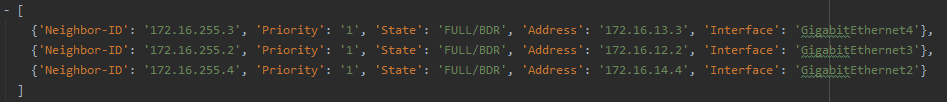
\includegraphics[scale=0.7]{\vorlagenOrdner/Bilder/Manual/OspfNeighbor.png}
					\caption{OSPF Neighbor Erwartungswert}
					\label{fig:OSPFNeighborErwartungswert}
				\end{center}
			\end{figure}

\subsection{Durchführung}
	Nachdem dass Inventar erstellt und die Testdefinitionen erfasst wurden,
	kann man das Programm starten.
	Falls die Option Skip-GUI aktiviert wurde, werden alle Tests in der Reihenfolge durchgeführt,
	in der sie in der Testdefinition angegeben wurden. 
	Falls dies nicht aktiviert wurde öffnet sich ein Grafikinterface.

	\newpage

	\subsubsection{GUI}
		Das GUI für die Definition der Test Reihenfolge besteht aus zweit Tabs:

		\begin{figure}[h!]
			\begin{center}
				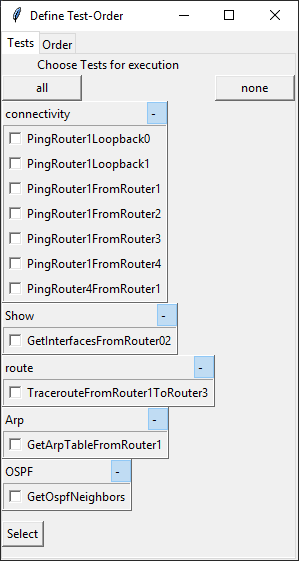
\includegraphics[scale=0.8]{\vorlagenOrdner/Bilder/Manual/GUI1.png}
				\caption{GUI Testauswahl}
			\end{center}
		\end{figure}

		Im ersten Tab werden alle Tests nach Gruppen sortiert angezeigt.
		Die Gruppierung ist diejenige, die in der Testdefinition angegeben wurde. 
		Hier kann der Benutzer auswählen welche Tests er ausführen möchte.
		Nachdem die Tests ausgewählt wurden weden mit dem Button 'Select' 
		alle ausgewählten Tests selektiert und man kann danach die Reihenfolge der
		selektierten Test im zweiten Tab einstellen.

		\newpage

		\begin{figure}[h!]
			\begin{center}
				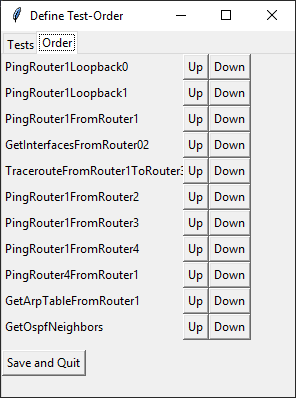
\includegraphics[scale=0.8]{\vorlagenOrdner/Bilder/Manual/GUI2.png}
				\caption{GUI Testreihenfolge}
			\end{center}
		\end{figure}

		Im zweiten Tab werden alle selektierten Tests angezeigt und der Benutzer 
		kann mit den jeweiligen Buttons die Reihenfolge bestimmen.
		Nachdem der Benutzer mit der Reihenfolge zufrieden ist,
		kann mit dem Button 'Save and Quit' das GUI beendet werden.
		Alle selektierten Tests werden nun in der angegebenen Reihenfolge durchgeführt.

	\newpage
		

	\subsubsection{Test Resultate}
		Die Resultate der jeweiligen Durchführungen werden in der Konsole angezeigt 
		und zusätzlich noch in einem File gespeichert.
		Bestandene Tests werden nur mit ihrem Namen und dem Vermerk, dass der Test bestanden ist,
		angegeben. 
		Nicht bestandene Tests haben den Testnamen, das erwartete Ergebniss und das tatsächliche
		Ergebniss für einen soll-ist-Vergleich.

		Die Abbildung~\ref{fig:ChooseTestGui} zeigt eine komplette Durchführung des Programms mit elf bestandenen
		Tests und null nicht bestandenen Tests: 


		\begin{figure}[h!]
			\begin{center}
				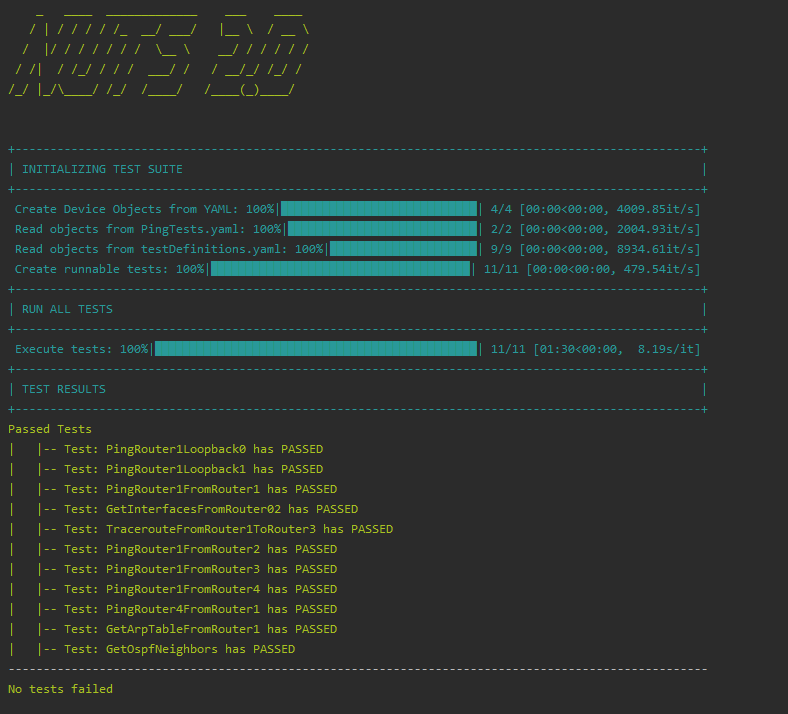
\includegraphics[scale=0.8]{\vorlagenOrdner/Bilder/Manual/ConsoleGUI.png}
				\caption{Programmausführung im PyCharm}
				\label{fig:ChooseTestGui}
			\end{center}
		\end{figure}

		\newpage

		Das File, in dem der Testreport abgespeichert wird, befindet sich unter: 
		'Resources/Inventory/TestResults/results.txt'.

		\begin{figure}[h!]
			\begin{center}
				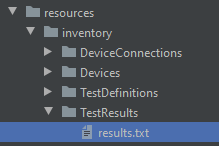
\includegraphics[scale=1.0]{\vorlagenOrdner/Bilder/Manual/TestResults_txt.png}
				\caption{Position Testresultate}
			\end{center}
		\end{figure}

		In dem File wird zuerst der Zeitstempel der Testdurchführung angegeben, 
		danach werden zuerst die bestandenen Tests und am Schluss die nicht bestandenen Tests angezeigt.
		Bei den nicht bestandenen Tests werden zusätzlich noch das erwartete und das tatsächliche
		Resultat angezeigt.

		\begin{figure}[h!]
			\begin{center}
				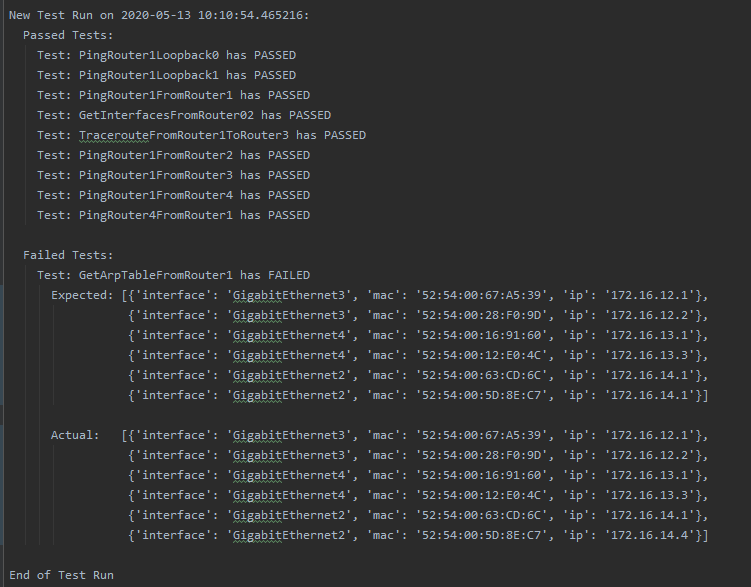
\includegraphics[scale=0.8]{\vorlagenOrdner/Bilder/Manual/TestResults.png}
				\caption{Testresultate.txt}
			\end{center}
		\end{figure}

		\newpage

\subsection{Neue Tests hinzufügen}
	Falls der Benutzer eigene Tests hinzufügen möchte,
	 müssen an folgenden Orten änderungen vorgenommen werden:

	\subsubsection{Conctrete Tests}
		Die konkreten Tests befinden sich unter 'nuts/testcreation/concretetests'
		In diesem Ordner muss ein neues Python-File angelegt werden.
		Im File wird der Test als Klasse implementiert.
		Es ist darauf zu achten, dass das Basisinterface 'NetworkTestStrategyInterface' 
		von der Testklasse implementiert wird, um davon die grundlegenden Funktionalitäten
		zu erben.

		\begin{figure}[h!]
			\begin{center}
				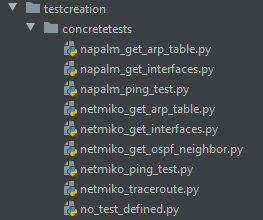
\includegraphics[scale=1.0]{\vorlagenOrdner/Bilder/Manual/concretetests.png}
				\caption{Position konkrete Netzwerktests}
			\end{center}
		\end{figure}

		Nach der Erstellung muss der Test geschrieben werden.
		Dazu wird in der \_\_init\_\_ Methode die Funktion self.nr. = InitNornir() aufgerufen
		und darin die benötigten Parameter übergeben.

		In der Methode run\_test(): wird angegeben, welches Nornir-Plugin mit welchem Task
		verwendet wird, z.B. task=napalm\_get.
		
		In der set\_result() Methode wird die Logik für das Parsen des Rückgabewerts des Tests
		implementiert. 
		Es ist darauf zu achten, dass dabei das Resultat in ein einheitliches Format gebracht 
		wird, so dass man in der evaluate\_result() Methode das erwartete Ergebnis möglichst 
		mit einem == zum tatsächlichen Ergebnis vergleichen kann.
		Falls dies nicht möglich ist, muss im evaluate\_result() zusätzlich Logik implementiert
		werden, um die Resultate zu vergleichen.

		Mehr Informationen, welche Begehle mit Nornir ausgeführt werden können, findet man 
		auf: \newline \url{https://nornir.readthedocs.io}

		Informationen zum Napalm-Treiber findet man auf: \url{https://napalm.readthedocs.io}

		Die bereits erstellten Tests können als Vorlage für weitere Testimplementationen verwendet 
		werden.
		
	\subsubsection{Network Test Strategy Factory}
		Die Network Test Strategy Factory implementiert die Logik, nach der die Tests ausgewählt 
		und instanziert werden.
		Dafür werden sämtliche Tests in einer test\_map gespeichert. 
		Die test\_map ist ein Dictionary von Dictionaries und hat als äusseren Key 
		den Befehl, welcher Test ausgeführt werden soll und als inneren Key die Connection,
		die für den Test verwendet wird. 
		Als Value ist die konkrete Klasse eingetragen, die für den Test instanziert werden soll.
		Gibt es für eine Kombination aus Command-Connection keinen konkreten Test, 
		muss hier statt der Testklasse ein 'None' angegeben werden. 
		Falls in der Instanzierungslogik ein Test, welcher in der Testdefinition angegeben wurde,
		nicht existiert, wird stattdessen ein NoTestDefined-Test instanziert, welcher 
		in der Evaluation immer 'nicht bestanden' zurückgibt mit der Anmerkung, dass dieser
		Test noch nicht erstellt wurde.

		Die Abbildung~\ref{fig:TestMap} zeigt die test\_map mit den oben beschriebenen Werten.

		\begin{figure}[h!]
			\begin{center}
		        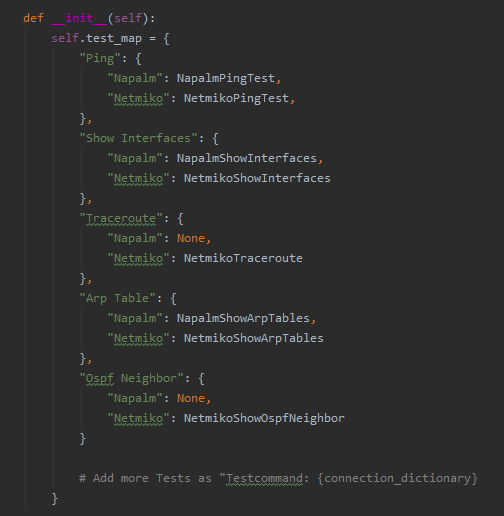
\includegraphics[scale=1.0]{\vorlagenOrdner/Bilder/Manual/strategyfactory.png}
				\caption{TestMap in der TestStrategyFactory}
				\label{fig:TestMap}
			\end{center}
		\end{figure}
        
\end{document}